\documentclass[]{beamer}
\usetheme[block=fill,progressbar=frametitle,numbering=none]{metropolis}
% Paquetes de la ams
\usepackage{amsmath,amsthm,amssymb,amsfonts}
% Codificacion UTF-8
\usepackage[utf8]{inputenc}
% Tablas e imagenes en espaniol
\usepackage[spanish,es-tabla]{babel}
% Mejores graficos
\usepackage{graphicx}
% tablas mas lindas
\usepackage{booktabs}
% Links a urls
\usepackage{url}
% Linkear referencias en pdfs
\usepackage{hyperref}
% Texto mas lindo para los pie de figura
\usepackage[margin=10pt,font=small,labelfont=bf, labelsep=endash]{caption}

% Citas
\usepackage[backend=biber,style=ieee]{biblatex}
\addbibresource{biblio.bib}

% Codigo
\usepackage{listings}

% Dir tree
\usepackage{dirtree}

% Pagina en blanco cuando ha
\usepackage{emptypage}

\definecolor{A11}{HTML}{B2DF8A}
\definecolor{A12}{HTML}{33A02C}
\definecolor{A23}{HTML}{FDBF6F}
\definecolor{A24}{HTML}{FF7F00}
\definecolor{B15}{HTML}{FB9A99}
\definecolor{B16}{HTML}{E31A1C}
\definecolor{B27}{HTML}{A6CEE3}
\definecolor{B28}{HTML}{1F78B4}

% Ejemplos, observaciones y teorema
\theoremstyle{definition}
\newtheorem{exa}{Ejemplo}[section]
\newtheorem*{obs}{Observación}
\newtheorem{que}{Pregunta}[section]
\newtheorem{dex}{Definicion}[section]

\author{Francisco Nemiña}
\title{Nivel 2: herramientas de teledetección cuantitativa}
\subtitle{El espectro electromagnético}
\institute{Unidad de Educación y Formación Masiva \\ Comisión Nacional de Actividades Espaciales}
\date{}
\graphicspath{{./figs/}}

\begin{document}

\maketitle

\begin{frame}{Table of contents}
  \setbeamertemplate{section in toc}[sections numbered]
  \tableofcontents[hideallsubsections]
\end{frame}

\section{Espacio espectral}
\begin{frame}{Discretización de la firma espectral}
  Hasta ahora la firma espectral es continua. Estudiemos que le pasa cuando el sensor la mide.
\end{frame}
%--- Next Frame ---%

\begin{frame}{Respuesta espectral}
  \begin{block}{Definición}
    Hablamos de la \emph{respuesta espectral de un sensor} cuando hablamos de como mide la luz que le llega al mismo en el dominio espectral.
  \end{block}
\end{frame}
%--- Next Frame ---%

\begin{frame}[t]{Respuesta espectral}
    \begin{exampleblock}{Ejemplo}
        \begin{figure}
            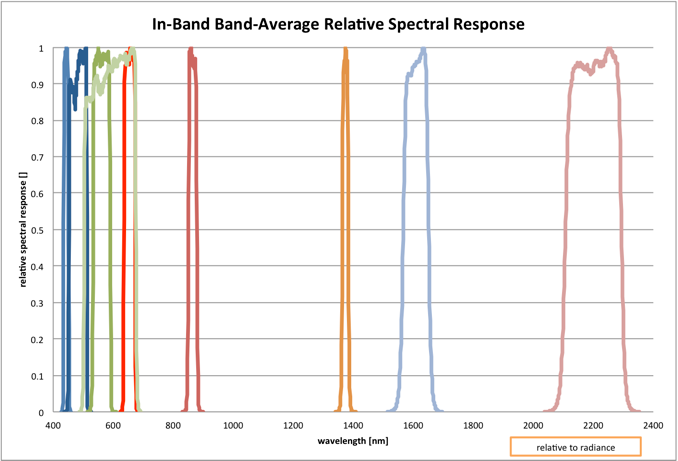
\includegraphics[width=0.67\textwidth]{AllBandsRSR.png}
            \caption{Respuestas espectrales de las bandas de Landsat 8.\footfullcite{barsi2014spectral}}
        \end{figure}
    \end{exampleblock}
\end{frame}
%--- Next Frame ---%

\begin{frame}{Respuesta espectral}
  Matematicamente, cuando un sensor mide la luz reflejada por un parche en el suelo esta haciendo un promedio pesado. Es decir:
  \begin{block}{Definición}
    El valor de brillo tomado por un sensor esta dado por
    \begin{equation}
        L_{j} =\frac{\int s_j(\lambda) L_\lambda d\lambda}{\int s_j(\lambda) d\lambda}.
    \end{equation}
  \end{block}
  esto para cada una de las N bandas de un sensor.
\end{frame}
%--- Next Frame ---%

\begin{frame}{Respuesta espectral}
  \begin{block}{Observación}
  \begin{itemize}
  \item El centro y el semi-ancho de un filtro nos permiten definir el centro de la banda y la correspondiente resolución espectral de la misma.
  \item En conclusión, al terminar el día la firma espectral queda discretizada según el número de bandas que usemos.
  \end{itemize}
  \end{block}
\end{frame}
%--- Next Frame ---%

\begin{frame}{Pixeles}
  Cada píxel va a tener asociado distintos valores de brillo, uno por banda de adquisición. \pause
  \begin{block}{Definición}
    Hablamos de un vector píxel al vector construido como
    \begin{equation}
      p = (\rho_1, \ldots ,\rho_N)
    \end{equation}
  \end{block}
\end{frame}
%--- Next Frame ---%

\begin{frame}{Píxeles - vectores}
  \begin{exampleblock}{Ejemplo}
    \begin{figure}
      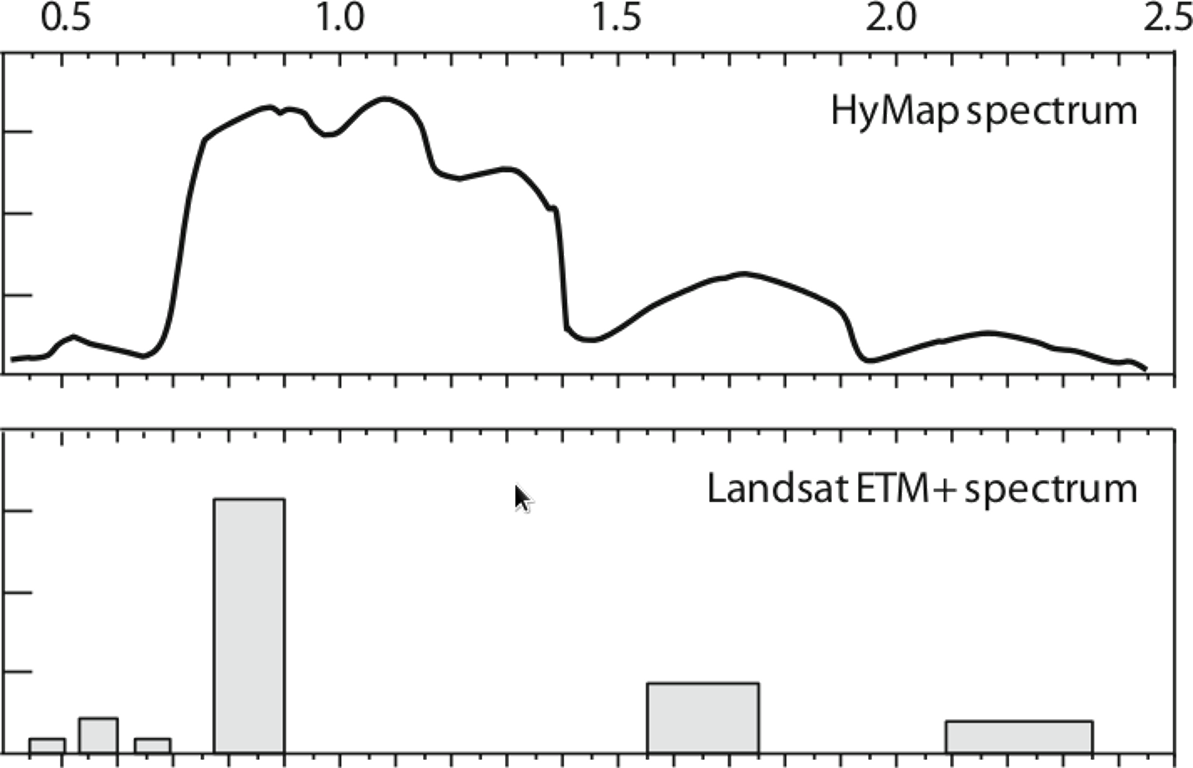
\includegraphics[width=0.6\textwidth]{elandsat.png}
    \end{figure}
  \end{exampleblock}
\end{frame}
%--- Next Frame ---%

\begin{frame}{Vectores}
  \begin{exampleblock}{Ejemplo}
    \begin{figure}
      \includegraphics[width=0.5\textwidth]{vector-3.png}
      \caption{Espacio espectral con 3 componentes y dos bandas. \footfullcite{richards2013remote}}
    \end{figure}
  \end{exampleblock}
\end{frame}
%--- Next Frame ---%


\begin{frame}{Espacio espectral}
  \begin{block}{Definición}
    Llamaremos \emph{espacio espectral} al espacio donde viven todos los vectores píxeles.
  \end{block}
\end{frame}
%--- Next Frame ---%

\end{document}
